\newpage
\section{Distributed Database Concepts}

% Distributed Databases
\subsection{Distributed Databases}

I dati utilizzati nelle infrastrutture dei big data \hl{devono essere ACID}. Queste infrastrutture sono \hl{composte da nodi che collaborano per compiere un task}. In queste infrastrutture andremo a distribuire le risorse sui nodi che cooperano in modo da avere \hl{ridondanza di dati}.

Esiste una \hl{relazione logica tra questi database connessi}, ma non tutti i nodi devono essere omogenei quindi possiamo al concetto di \hl{DISTRIBUTED DBMS} che deve gestire l'avere modelli dati connessi. 

Per quanto riguarda \hl{le query bisognera' riorganizzarle} per poter gestire i nodi distribuiti.


% Forme di trasparenza
\subsection{Forme di trasparenza}

Abbiamo varie forme di \hl{trasparenza rispetto all'utente}:

\begin{itemize}
    \item \hl{organizzazione dei dati}:

        \begin{itemize}
            \item local transparency
            \item naming transparency
        \end{itemize}
    
    \item \hl{ridondanza}: usata per ridurre la mancanza del servizio
    
    \item \hl{frammentazione dei dati}:

        \begin{itemize}
            \item \textbf{partizione orizzontale}: abbiamo una partizione delle tuple. La struttura dati è la stessa ma cambiano i dati salvati
            
            \begin{figure}[H]
            \centering
            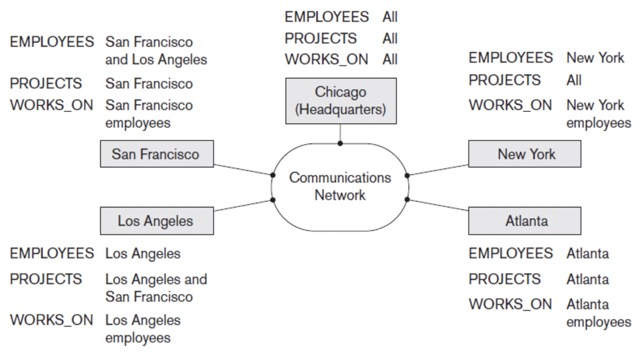
\includegraphics[scale=0.4]{partoriz.jpeg}
            \caption{Partizione orizzontale di un db} 
            \label{partoriz}
            \end{figure}

            \item \textbf{partizione verticale}: frammentazione del modello dati attraverso la partizione degli attributi che possono essere dislocati su più nodi
        \end{itemize}
    
\end{itemize}


% Affidabilità e disponibilità
\subsection{Affidabilità e disponibilità}

Per poter rispettare affidabilità e disponibilità usiamo la \hl{ridondanza}.

Eseguiamo una distribuzione dei dati \hl{per avere la possibilita' di scalare i dati in modo orizzontale o verticale} a seconda dell'uso che dobbiamo farne. Parliamo di:

\begin{itemize}
    \item \hl{horizzontal scalability}: poter \textbf{espandere il numero di nodi} del sistema
    \item \hl{vertical scalability}: poter espandere la \textbf{capacità di un singolo nodo}
    \item \hl{partition tolerance}: il sistema è \textbf{capace di operare anche se partizionato}
\end{itemize}


% Autonomia
\subsection{Autonomia}

La caratteristica principale della distribuzione è l'\hl{autonomia di ogni nodo rispetto agli altri}, quindi lo deve essere anche il loro contenuto, tenendo conto di:

\begin{itemize}
    \item \hl{design autonomy}: rappresenta indipendenza dei modelli dei dati e la \textbf{gestione delle transazioni tra i nodi}
    \item \hl{communication autonomy}: dà la possibilità di condividere le informazioni
    \item \hl{execution autonomy}: mi assicura che posso \textbf{eseguire una query}
\end{itemize}

Il \hl{vantaggio delle architetture distribuite} è una migliore facilità di sviluppo, disponibilità e performance.


% Frammenti
\subsection{Frammenti}

I frammenti sono le \hl{unita' logiche dei database} e possono essere:

\begin{itemize}
    \item \hl{frammentazione orizzontale}: divide le relazioni in orizzontale (\textbf{tuple})
    \item \hl{frammentazione verticale}: divide le relazioni in verticale (\textbf{colonne})
    \item \hl{frammentazione orizzontale completa}: se tramite \textbf{union} possiamo ricostruire la nostra lezione completamente
    \item \hl{frammentazione verticale completa}: usiamo la \textbf{join}
\end{itemize}

Spesso nella ricostruzione di un db possiamo trovare sia frammentazioni verticali che orizzontali, parliamo allora di \hl{frammentazione dello schema}.

Un DDBMS è in grado di gestire una frammentazione usando un \hl{ALLOCATION SCHEMA} che \hl{specifica come i frammenti del db sono distribuiti su quali nodi}.

Quando abbiamo dei dati possiamo avere la necessità di ridondanza. Questo non è il metodo migliore per chi si occupa di \hl{grandi moli di dati}, infatti bisognerà fare delle \hl{repliche a caldo che ogni tempo t} su un altro sito. In questi casi \hl{ci viene in soccorso il database journal} che \hl{tiene traccia dei log/modifiche} fatte al db, andando a prevenire eventuali errori dato che si potrà accedere ad una versione immediatamente precedente dei dati.

Potremo avere delle \hl{repliche totali o parziali}, replicando struttura e dati a secondo dello schema di replica presente del DDBMS.


% Problemi per DDBMS
\subsection{Problemi per DDBMS}

Potrebbero essere:

\begin{itemize}
    \item eccessive copie dei dati
    \item \hl{two phase commit}: dove un nodo quando ne aggiorna un altro ha la possibilità che fallisca e gli sia mandato un ACK -1, in questo casi bisognerà rincominciare tutto dall'inizio
\end{itemize}

Nella gestione delle ridondanza si utilizza un \hl{sito primario} che può essere sostituito, nel caso di malfunzionamenti, da uno secondario, andando a \hl{gestire le tabelle in modo parallelo}. Per capire chi sarà il nuovo responsabile del locking si usa un \hl{sistema a voto}. 







Un sistema distribuito `e un sistema che ha risorse di elabo- razione che possono essere dislocati su nodi che potrebbero anche essere geograficamente distanti. La relazione che esiste tra questi diversi nodi `e di tipo logico, tutti questi sono omoge- nei. Il principio principale `e che l’utente finale, che pu`o essere anche un programmatore, non deve accorgersi che il database `e di tipo distribuito. La trasparenza si puo` applicare sia sotto il punto di vista della locazione fisica che anche dal punto di vista del naming delle tabelle, ovvero non c’`e bisogno che io abbia chiamato le tabelle nello stesso modo. Altre propriet`a importanti sono la Replication Transparency che permette di replicare i dati nel caso di disservizio, l’utente finale ovvia- mente non si rendera` conto di questo processo. Anche la Fragmentation Transparency `e un metodo di frammentazio- ne che puo` essere orizzontale se abbiamo su due database diversi la stessa struttura dati ma differenti righe e verticale se disponiamo di due strutture dati differenti ma in relazione logica tra loro (come se stessimo tagliando verticalmente la tabella).


img


Questo esempio rappresenta una frammentazione orizzon- tale (sharding),parliamo di frammentazione orizzontale com- pleta se siamo in grado attraverso l’operazione di union di riavere la relazione iniziale completa (in generale per lavora- re sulle colonne utilizziamo l’operazione di join, sulle righe la union). I motivi per cui si vuole distribuire un database so- no differenti, dobbiamo essere in grado di fornire avaiability e Raliability ovvero delle caratteristiche relative alla dispo- nibilit`a del dato ed alla robustezza della struttura oltre che per questioni di scalabilit`a. Si parla di Partition Tolerance quando il sistema `e in grado di operare nonostante sia par- tizionato. Questo `e derivato direttamente dal cut teorem, questo afferma che un sistema partizionato puo` funzionare come se non lo fosse ma non pu`o garantire consistenza e la disponibilit`a insieme, a differenza dei sistemi non partizionati che utilizzano un sistema ACID: Atomicit`a , consistenza, in- tegrit`a, durabilit`a dei dati, propriet`a disponibili facilmente in un database relazionale non distribuito. Altra caratteristica importante in un sistema frammentata `e quella che assicu- ra che un nodo pu`o decidere autonomamente se condividere in suo dato con altri nodi. In un sistema frammentato ogni tabella dovra` necessariamente avere la sua chiave primaria e queste chiavi primarie saranno sfruttate come parametro per effettuare una join. La frammentazione viene gestita attra- verso quello che viene chiamato allocation schema e ti fornisce informazioni riguardanti la posizione dei frammenti sui vari nodi. Un altro fattore importante `e la replicabilita` del si- stema, quindi un sistema frammentato deve essere facilmente ricostruibile. Altro meccanismo importante `e quello del two phase commit, supponendo di avere un database main e uno doppione e supponiamo di voler eseguire una transazione, in questo caso dovr`o ricevere non uno ma due messaggi di modi- fica effettuata con successo, se qualcosa dovesse andare storto necessito di effettuare un rollback su entrambe i database e quindi tornare alle condizioni precedenti. Generalmente esi- ste un sistema main a cui ci si rivolge e se questo va down allora l’infrastruttura sara` responsabile di reindirizzare al ser- ver che permettere l’accesso ai dati che abbiamo richiesto al main, quindi questo server dovr`a avere una replica di quei dati richiesti in precedenza. Esistono differenti metodi di scelta di questi server se un server main va offline. Adesso poniamoci la domanda: quali sono i passi che vengono realizzati quando noi eseguiamo una query in ambiente distribuito ? Analiz- ziamo la prima tecnica importante che `e il query mapping, questo `e il termine che si usa per rappresentare la metodolo- gia che permette di capire quali dati vengono utilizzati dalla query e dove questi dati si trovano sui vari frammenti. Una volta effettuata la mappatura il dbms effettuer`a la query in modo decentralizzato, quindi questa verr`a spezzata, svolta e riorganizzata. Ovviamente il ddbms supporta l’ottimizzazio- ne delle query. Nell’ottimizzazione sono importanti gli indici, questi sono degli strumenti messi a disposizione del dbms che permettono l’ottimizzazione delle query, indicano i valori piu` richiesti su un database. E` norma apportare degli indici sulle chiavi primarie ed ereditate. La procedura di inserimento e utilizzo degli indici pu`o velocizzare il processo svolto da una query anche di 100 o 1000 volte. L’obiettivo dell’ottimizza- zione sulle query `e quello di ridurre la quantita` di dati che io devo trasmettere al fine di ottenere il risultato. Utilizziamo un costrutto particolare che `e la semi-join, questa riduce il numero di tuple che io mi trasmetto mandando soltanto la co- lonna di join e prendendo unicamente i valori che mi vengono dalla join della tabella di partenza. L’omogeneita` dei data influenza questi parametri di ottimizzazione. Altro concetto molto utilizzato in ambito dei ddbms relazionali `e quello del database federato. Questo database federato funziona in questo modo: ho un modello dati condiviso da tutti ma i sin- goli nodi dispongono di modelli dati indipendenti, quindi ogni nodo mantiene uno schema generale che permette di comu- nicare con gli altri, ma a livello individuale il nodo pu`o pre- sentare comportamenti diversi rispetto ai suoi simili. Si pu`o classificare il database distribuito su 3 differenti dimensioni:

\begin{itemize}
    \item Autonomia
    \item Distribuzione
    \item Eterogeneità
\end{itemize}

La rappresentazione dei dati `e delineata dal data-model e dal data-set. Nella figura seguente `e possibile visualizzare le differenti dimensioni:

